%package list
\documentclass{article}
\usepackage[top=3cm, bottom=3cm, outer=3cm, inner=3cm]{geometry}
\usepackage{multicol}
\usepackage{graphicx}
\usepackage{url}
%\usepackage{cite}
\usepackage{hyperref}
\usepackage{array}
%\usepackage{multicol}
\newcolumntype{x}[1]{>{\centering\arraybackslash\hspace{0pt}}p{#1}}
\usepackage{natbib}
\usepackage{pdfpages}
\usepackage{multirow}
\usepackage[normalem]{ulem}
\useunder{\uline}{\ul}{}
\usepackage{svg}
\usepackage{xcolor}
\usepackage{listings}
\lstdefinestyle{ascii-tree}{
    literate={├}{|}1 {─}{--}1 {└}{+}1 
  }
\lstset{basicstyle=\ttfamily,
  showstringspaces=false,
  commentstyle=\color{red},
  keywordstyle=\color{blue}
}
%\usepackage{booktabs}
\usepackage{caption}
\usepackage{subcaption}
\usepackage{float}

\newcolumntype{M}[1]{>{\centering\arraybackslash}m{#1}}
\newcolumntype{N}{@{}m{0pt}@{}}


%%%%%%%%%%%%%%%%%%%%%%%%%%%%%%%%%%%%%%%%%%%%%%%%%%%%%%%%%%%%%%%%%%%%%%%%%%%%
%%%%%%%%%%%%%%%%%%%%%%%%%%%%%%%%%%%%%%%%%%%%%%%%%%%%%%%%%%%%%%%%%%%%%%%%%%%%
\newcommand{\itemEmail}{jmamanices@unsa.edu.pe}
\newcommand{\itemStudent}{Jhonatan Benjamin Mamani Céspedes}
\newcommand{\itemCourse}{Programación Web 2}
\newcommand{\itemCourseCode}{1702122}
\newcommand{\itemSemester}{III}
\newcommand{\itemUniversity}{Universidad Nacional de San Agustín de Arequipa}
\newcommand{\itemFaculty}{Facultad de Ingeniería de Producción y Servicios}
\newcommand{\itemDepartment}{Departamento Académico de Ingeniería de Sistemas e Informática}
\newcommand{\itemSchool}{Escuela Profesional de Ingeniería de Sistemas}
\newcommand{\itemAcademic}{2024 - A}
\newcommand{\itemInput}{Del 20 Mayo 2024}
\newcommand{\itemOutput}{Al 26 Mayo 2024}
\newcommand{\itemPracticeNumber}{01}
\newcommand{\itemTheme}{Modelos en Django}
%%%%%%%%%%%%%%%%%%%%%%%%%%%%%%%%%%%%%%%%%%%%%%%%%%%%%%%%%%%%%%%%%%%%%%%%%%%%
%%%%%%%%%%%%%%%%%%%%%%%%%%%%%%%%%%%%%%%%%%%%%%%%%%%%%%%%%%%%%%%%%%%%%%%%%%%%

\usepackage[english,spanish]{babel}
\usepackage[utf8]{inputenc}
\AtBeginDocument{\selectlanguage{spanish}}
\renewcommand{\figurename}{Figura}
\renewcommand{\refname}{Referencias}
\renewcommand{\tablename}{Tabla} %esto no funciona cuando se usa babel
\AtBeginDocument{%
	\renewcommand\tablename{Tabla}
}

\usepackage{fancyhdr}
\pagestyle{fancy}
\fancyhf{}
\setlength{\headheight}{30pt}
\renewcommand{\headrulewidth}{1pt}
\renewcommand{\footrulewidth}{1pt}
\fancyhead[L]{\raisebox{-0.2\height}{
\includegraphics[width=3cm]{img/logo_episunsa.png}}}
\fancyhead[C]{\fontsize{7}{7}\selectfont	\itemUniversity \\ \itemFaculty \\ \itemDepartment \\ \itemSchool \\ \textbf{\itemCourse}}
\fancyhead[R]{\raisebox{-0.2\height}{
\includegraphics[width=1.2cm]{img/logo_abet}}}
\fancyfoot[L]{Estudiante: Jhonatan Mamani}
\fancyfoot[C]{\itemCourse}
\fancyfoot[R]{Página \thepage}

% para el codigo fuente
\usepackage{listings}
\usepackage{color, colortbl}
\definecolor{dkgreen}{rgb}{0,0.6,0}
\definecolor{gray}{rgb}{0.5,0.5,0.5}
\definecolor{mauve}{rgb}{0.58,0,0.82}
\definecolor{codebackground}{rgb}{0.95, 0.95, 0.92}
\definecolor{tablebackground}{rgb}{0.8, 0, 0}

\lstset{frame=tb,
	language=bash,
	aboveskip=3mm,
	belowskip=3mm,
	showstringspaces=false,
	columns=flexible,
	basicstyle={\small\ttfamily},
	numbers=none,
	numberstyle=\tiny\color{gray},
	keywordstyle=\color{blue},
	commentstyle=\color{dkgreen},
	stringstyle=\color{mauve},
	breaklines=true,
	breakatwhitespace=true,
	tabsize=3,
	backgroundcolor= \color{codebackground},
}

\begin{document}
	
	\vspace*{10px}
	
	\begin{center}	
		\fontsize{17}{17} \textbf{ Informe de Programación Web - Django \itemPracticeNumber}
	\end{center}
	\centerline{\textbf{\Large Tema: \itemTheme}}
	%\vspace*{0.5cm}	

	\begin{flushright}
		\begin{tabular}{|M{2.5cm}|N|}
			\hline 
			\rowcolor{tablebackground}
			\color{white} \textbf{Nota}  \\
			\hline 
			     \\[30pt]
			\hline 			
		\end{tabular}
	\end{flushright}	

	\begin{table}[H]
		\begin{tabular}{|x{4.7cm}|x{4.8cm}|x{4.8cm}|}
			\hline 
			\rowcolor{tablebackground}
			\color{white} \textbf{Estudiantes} & \color{white}\textbf{Escuela}  & \color{white}\textbf{Asignatura}   \\
			\hline 
			{\itemStudent \par \itemEmail} & \itemSchool & {\itemCourse \par Semestre: \itemSemester \par Código: \itemCourseCode}     \\
			\hline 			
		\end{tabular}
	\end{table}		
	
	\begin{table}[H]
		\begin{tabular}{|x{4.7cm}|x{4.8cm}|x{4.8cm}|}
			\hline 
			\rowcolor{tablebackground}
			\color{white}\textbf{Práctica} & \color{white}\textbf{Tema}  & \color{white}\textbf{Duración}   \\
			\hline 
			\itemPracticeNumber & \itemTheme & 04 horas   \\
			\hline 
		\end{tabular}
	\end{table}
	
	\begin{table}[H]
		\begin{tabular}{|x{4.7cm}|x{4.8cm}|x{4.8cm}|}
			\hline 
			\rowcolor{tablebackground}
			\color{white}\textbf{Semestre académico} & \color{white}\textbf{Fecha de inicio}  & \color{white}\textbf{Fecha de entrega}   \\
			\hline 
			\itemAcademic & \itemInput &  \itemOutput  \\
			\hline 
		\end{tabular}
	\end{table}
	
	\section{Tarea}
	\begin{itemize}		
            \item Instalación, el ambiente virtual
            \item Crear un proyecto Django en blanco
            \item Configuración
            \item Componentes integrados
            \item Primer componente de aplicación
            \item Crear objetos en Python Shell
            \item Nuevos campos en el modelo
	\end{itemize}
		
	\section{Equipos, materiales y temas utilizados}
	\begin{itemize}
            \item Sistema Operativo Windows 11 Home v 23H2 64 bits
            \item VIM x64 v9.1.
            \item Visual Studio Code x64 v1.89.1
            \item Git v2.45.0.
            \item Cuenta en GitHub con el correo institucional.
            \item Python v3.12.3.
            \item Entorno virtual.
            \item Django v5.0.6.
	\end{itemize}
	
	\section{URL de Repositorio Github}
	\begin{itemize}
            \item URL del Repositorio GitHub en donde se realiza el proyecto
            \item \url{https://github.com/JBenjamin01/pw2-django}
	\end{itemize}

    %%%%%%%%%%%%%%%%%%%% PRIMEROS PASOS %%%%%%%%%%%%%%%%%%%%
	
    \section{Creación del entorno virtual}

        \subsection{Entorno virtual}
        \begin{itemize}	
            \item Lo primero en realizarse fue crear un entorno virtual para instalar el paquete del framework Django.
            \item Así que lo primero fue crear dicho entorno, se usó lo siguiente (en Windows)
        \end{itemize}
 
        \begin{lstlisting}[language=bash,caption={Creación del entorno virtual}][H]
        $ virtualenv -p python3 python_env
        \end{lstlisting}

        \subsection{Activación}
        \begin{itemize}	
            \item Después de crearlo, se necesita activarlo. Para esto se usó lo siguiente:
	\end{itemize}

        \begin{lstlisting}[language=bash,caption={Activación del entorno virtual}][H]
        $ cd python_env
        $ .\Scripts\Activate.ps1
        \end{lstlisting}

        \begin{itemize}	
            \item Fuera del directorio del entorno virtual, se crea una carpeta que contendrá el proyecto:
	\end{itemize}
        \begin{lstlisting}[language=bash,caption={Directorio de trabajo del proyecto}][H]
        $ cd ..
        $ mkdir pw2-django
        \end{lstlisting}

        \subsection{Dependencias}
        \begin{itemize}	
            \item Finalmente, solo faltaba instalar las dependencias, en este caso, solo Django, con pip freeze revisamos si se instaló correctamente.
	\end{itemize}

        \begin{lstlisting}[language=bash,caption={Instalación del paquete DJango}][H]
        $ pip install Django
        \end{lstlisting}

        \begin{itemize}	
            \item Una vez instalado podemos proceder con el trabajo.
	\end{itemize}

    %%%%%%%%%%%%%%%%%%%% INICIO DEL PROYECTO %%%%%%%%%%%%%%%%%%%%
    \section{Creación del proyecto Django}
        \subsection{Configuración básica}
        \begin{itemize}
            \item Entonces, dentro de la ruta principal del proyecto, creo un nuevo proyecto en el cual trabajaré todo lo que se hizo en las diapositivas:
             
        \begin{lstlisting}[language=bash,caption={Inicio del proyecto}][H]
        $ cd pw2-django
        $ django-admin startproject listaContactos
        \end{lstlisting}
            
            \item Tras crear el proyecto se realiza una configuración simple en listaContactos/settings.py, según las diapositivas seguidas se deben modificar el idioma y la zona horaria.
            
        \begin{lstlisting}[language=bash,caption={Ingresando a settings.py}][H]
        $ vim listaContactos/listaContactos/settings.py
        \end{lstlisting}
            \item Modificamos la zona horaria y el idioma:

        \begin{lstlisting}[language=Python, caption={Configuración de idioma y zona horaria}]
        LANGUAGE_CODE = 'es'
                    
        TIME_ZONE = 'America/Lima'
                    
        USE_I18N = True
                    
        USE_TZ = True
        \end{lstlisting}

            \item El commit realizado fué el siguiente:

        \begin{figure}[H]
            \centering
            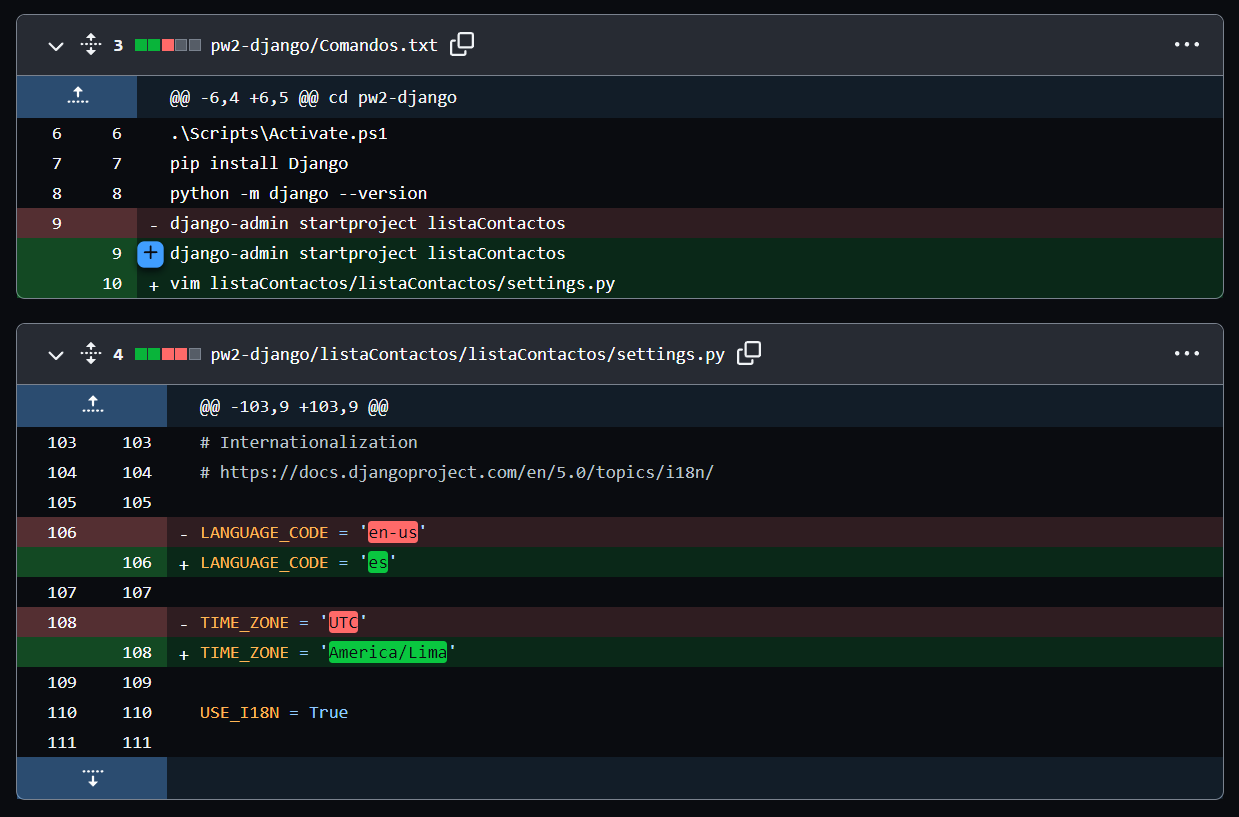
\includegraphics[width=0.7\linewidth]{img/Commit1.png}
            \caption{Commit de los cambios}
            \label{fig:enter-label}
        \end{figure}
        \end{itemize}

        \subsection{Servidor}
        \begin{itemize}
            \item Con este primer paso se revisa que el servidor pueda correr sin problema, entonces realizamos el siguiente comando:
        
        \begin{lstlisting}[language=bash,caption={Activación del servidor}][H]
        $ python manage.py runserver
        \end{lstlisting}
    
            \item Y una vez realizado esto, accedemos al enlace que nos da el servidor para verificar su funcionamiento, en \url{http://127.0.0.1:8000/}
        
        \begin{figure}[H]
            \centering
            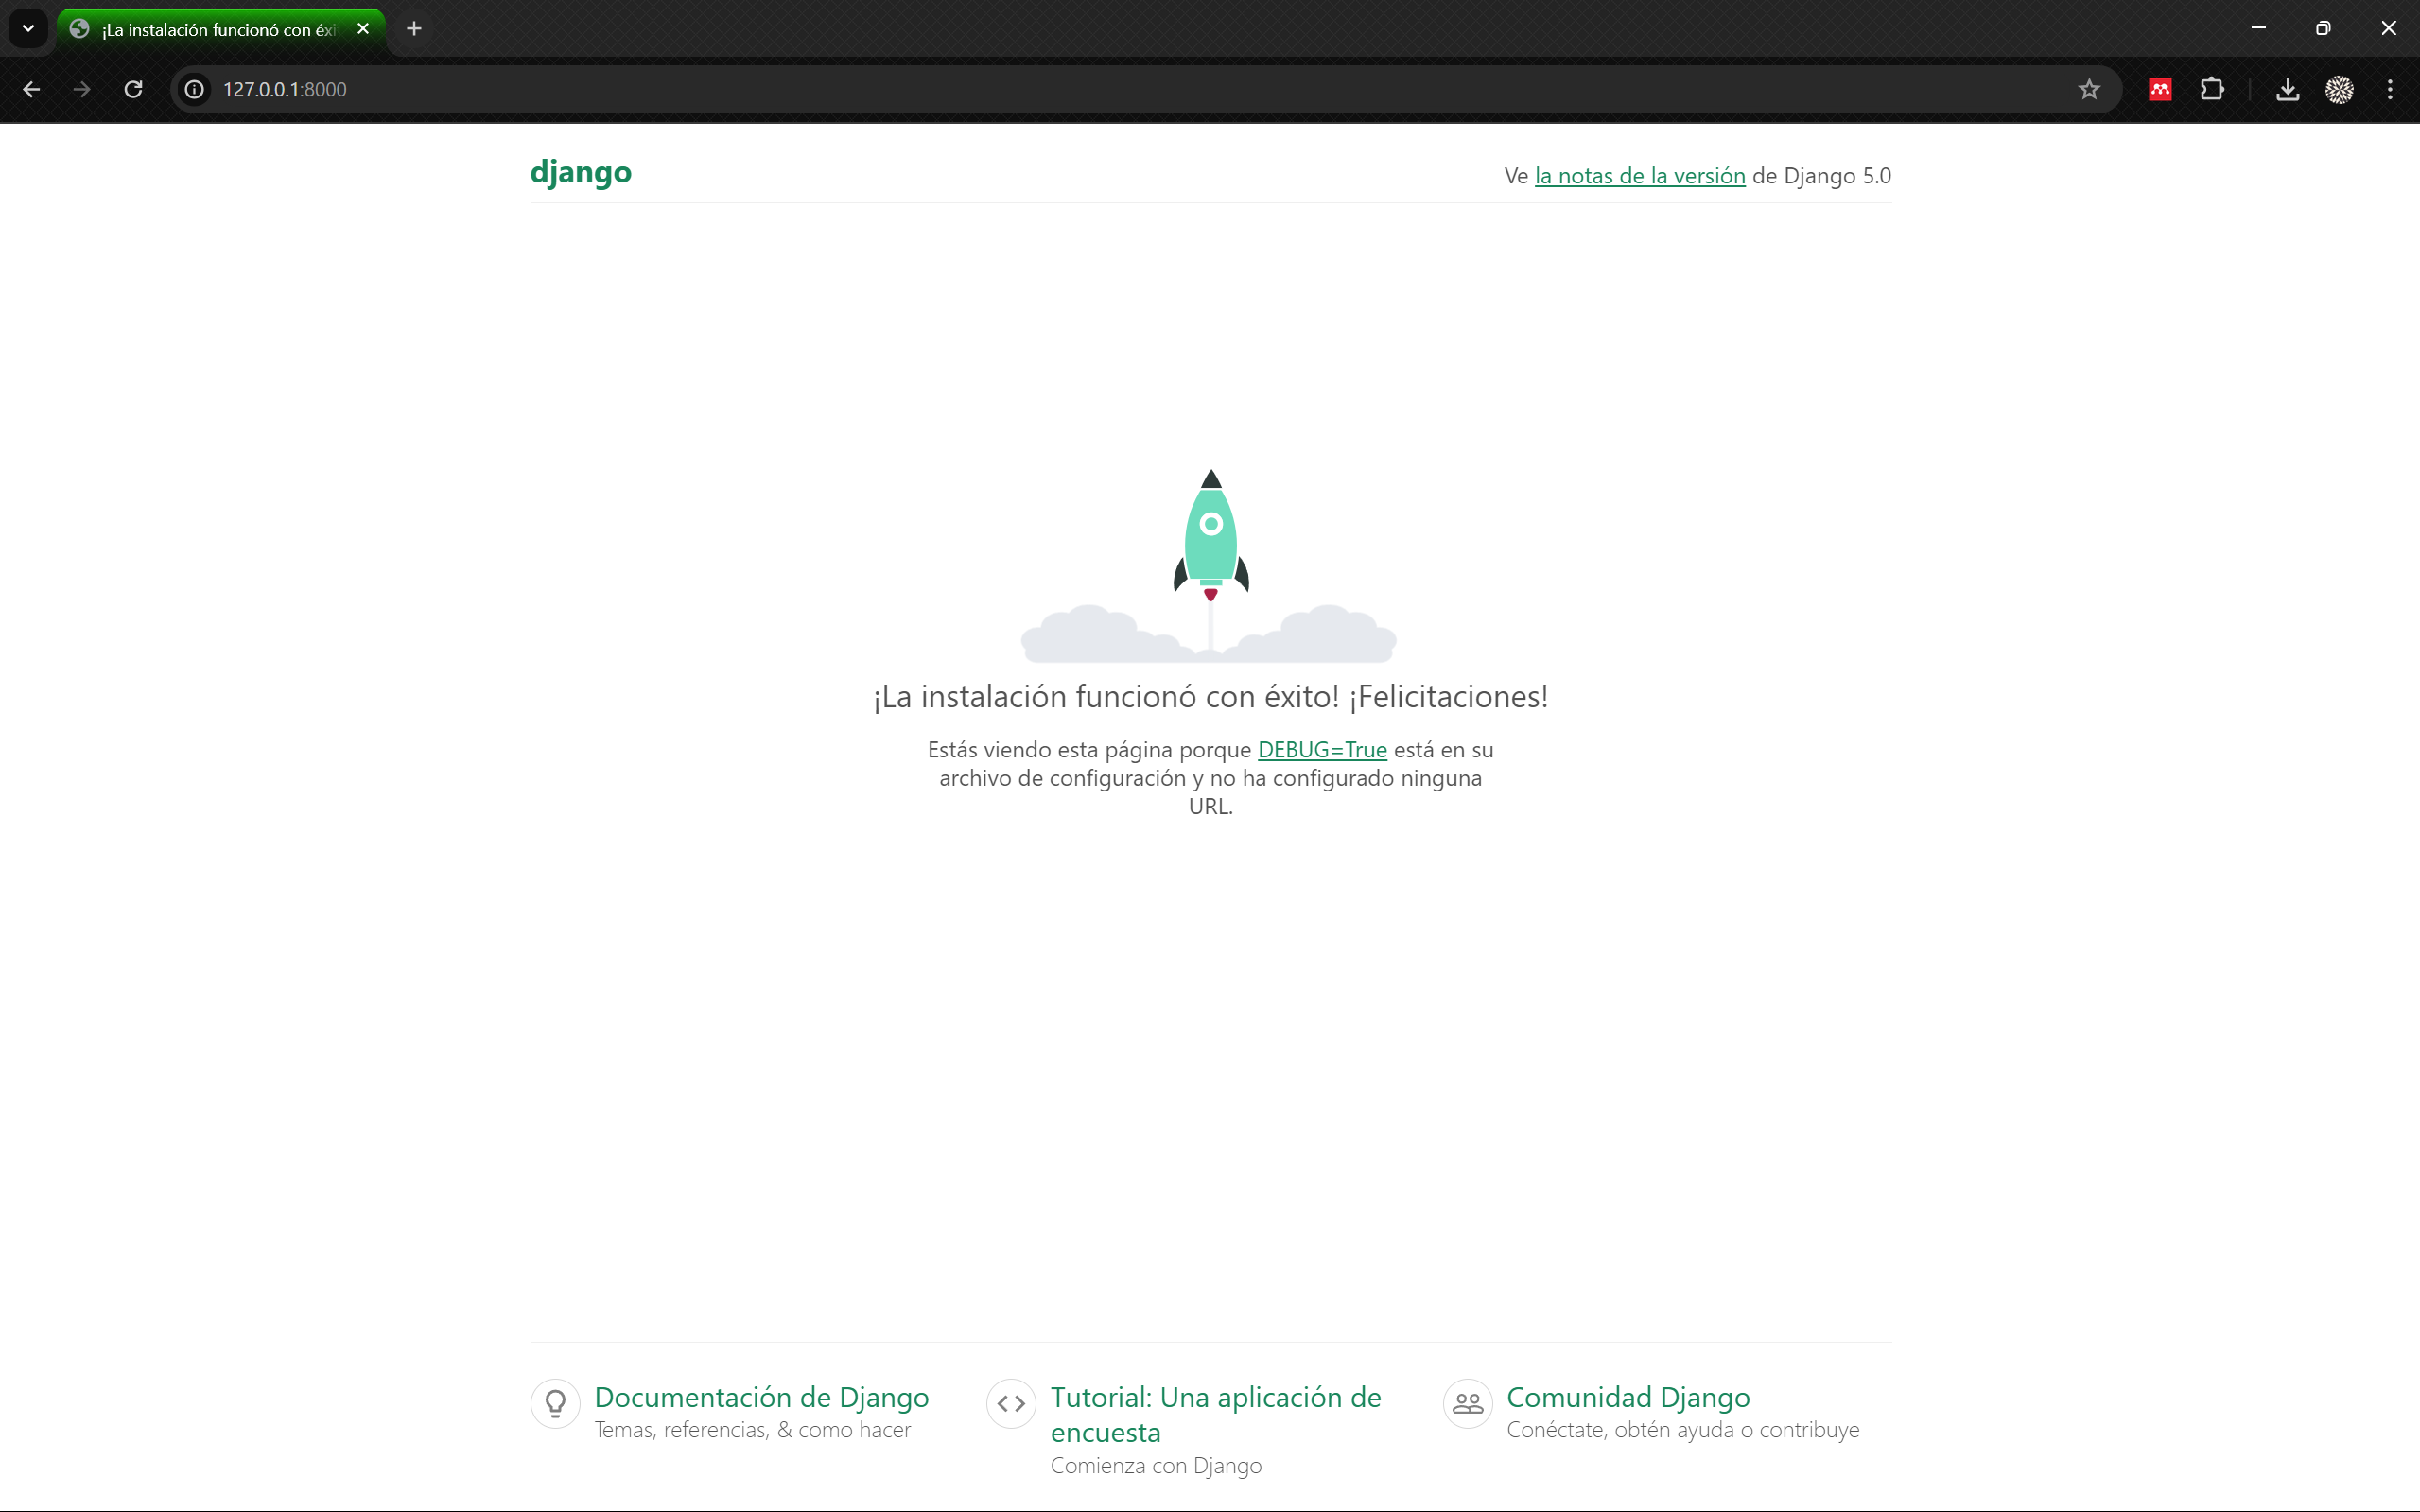
\includegraphics[width=1\linewidth]{img/Django_site.png}
            \caption{Página principal del servidor en Django}
            \label{fig:enter-label}
        \end{figure}

            \item Y efectivamente, parece no haber ningun problema con el servidor.
        \end{itemize}

    %%%%%%%%%%%%%%%%%%%% APPS %%%%%%%%%%%%%%%%%%%%
    
    \section{Creando la App 'personas'}
        \subsection{App}
        \begin{itemize}
            \item Entonces, ahora ubicados en el directorio dentro del proyecto, se procede a crear la primera app, en este caso, personas:        


        \begin{lstlisting}[language=bash,caption={Comando para crear la app personas}][H]
        $ django-admin startapp personas
            \end{lstlisting}
        \end{itemize}
        \subsection{Modelos}
        \begin{itemize}
            \item Con la nueva aplicación, se pueden editar los archivos propios de esta, el primer paso que se sigue es la creación del modelo Persona.
            \item Entonces, editamos el archivo models.py de la app recien creada:
        
        \begin{lstlisting}[language=bash,caption={Ingresando a models.py}][H]
        $ vim personas/models.py
        \end{lstlisting}

            \item Y creamos esta nueva clase Persona para asignarla como un nuevo modelo:
        
        \begin{lstlisting}[language=Python, caption={Modelo Persona}]
        from django.db import models
    
        # Create your models here.
        class Persona(models.Model):
            nombres = models.TextField()
            apellidos = models.TextField()
            edad = models.TextField()
        \end{lstlisting}
        
            \item Un paso importante es modificar el archivo settings.py en el registro de las apps de nuestro proyecto, entonces nos dirigimos a este archivo:

        \begin{lstlisting}[language=bash,caption={Ingresando a settings.py}][H]
        $ vim listaContactos/settings.py
        \end{lstlisting}
            \item Bajando hasta la parte de INSTALLED\_APPS, agregamos la aplicación que acabamos de crear al final de la lista:
        \begin{lstlisting}[language=Python, caption={Aplicaciones del proyecto}]
        # Application definition
    
        INSTALLED_APPS = [
            'django.contrib.admin',
            'django.contrib.auth',
            'django.contrib.contenttypes',
            'django.contrib.sessions',
            'django.contrib.messages',
            'django.contrib.staticfiles',
            'personas',
        ]
        \end{lstlisting}
        
            \item El commit realizado fué el siguiente:
            
        \begin{figure}[H]
            \centering
            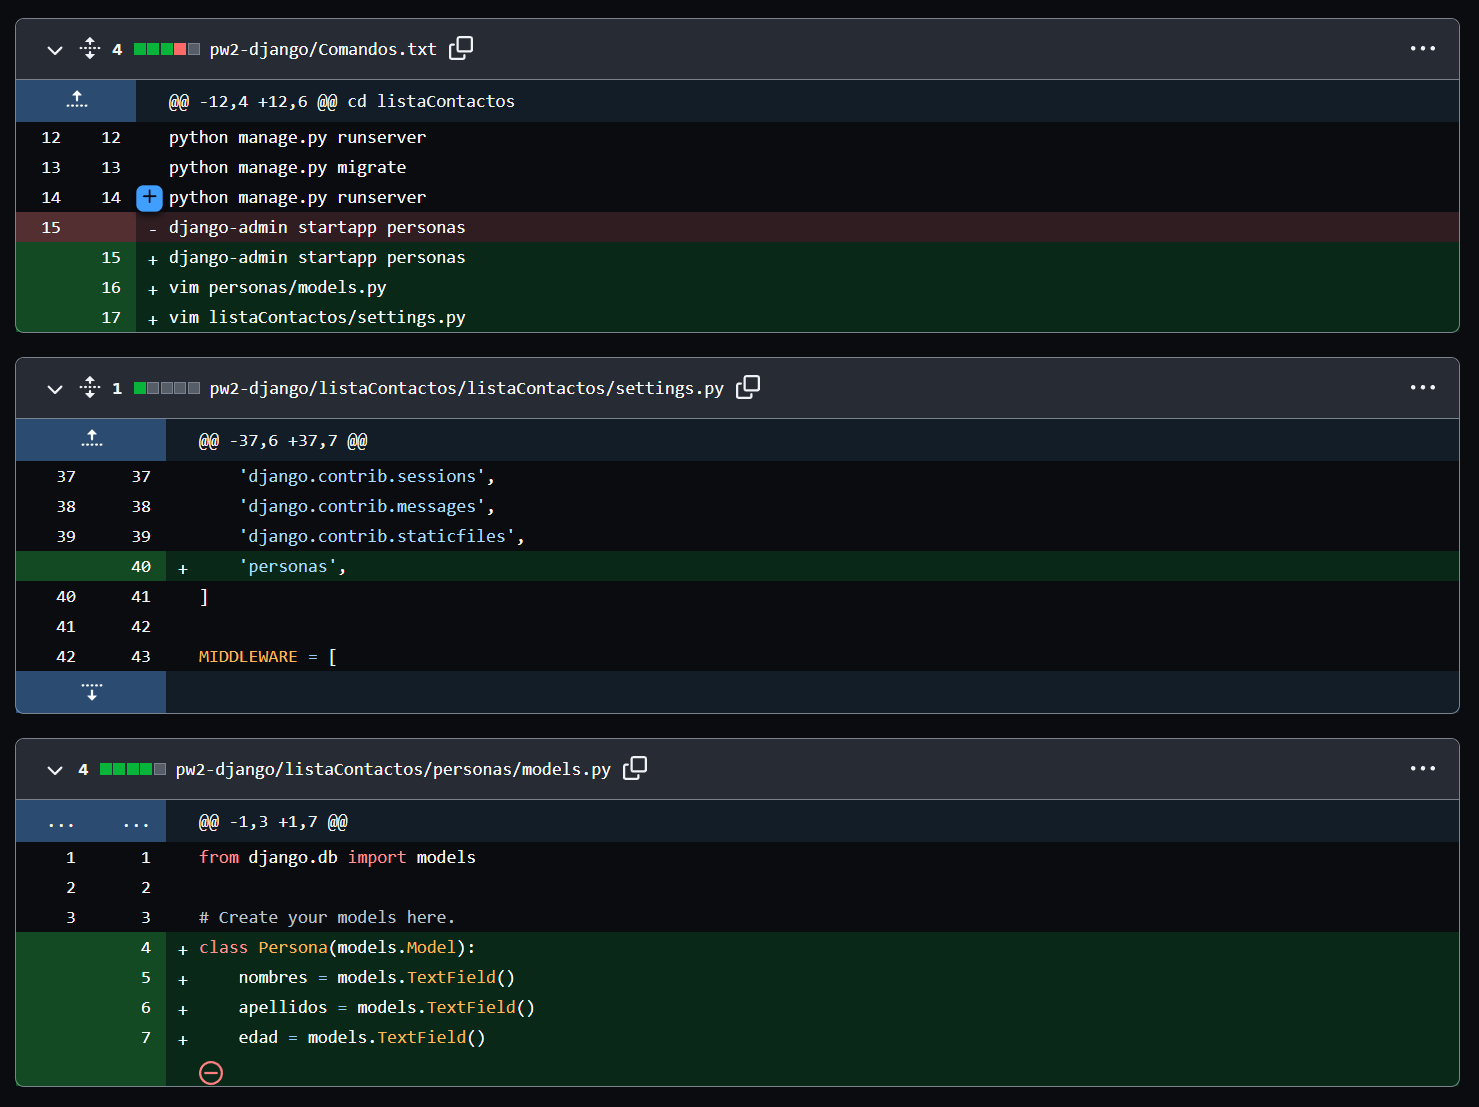
\includegraphics[width=0.7\linewidth]{img/Commit2.png}
            \caption{Commit de los cambios}
            \label{fig:enter-label}
        \end{figure}
        \end{itemize}
        
        \subsection{Migrations}
        \begin{itemize}
            \item Luego de haber realizado esta modificación a la aplicación de personas, añadiendo el nuevo modelo, se necesitan avisar sobre los cambios realizados y aplicarlos en nuestro proyecto. En los pasos de las diapositivas se siguen los siguientes comandos:
        
        \begin{lstlisting}[language=bash,caption={Makemigrations y migrate}][H]
        $ python manage.py makemigrations
        $ python manage.py migrate
        \end{lstlisting}

            \item Al ejecutarlos, se genera un nuevo archivo '0001\_initial.py' en la carpeta migrations de la app personas, esto se ve en el siguiente commit:

        \begin{figure}[H]
            \centering
            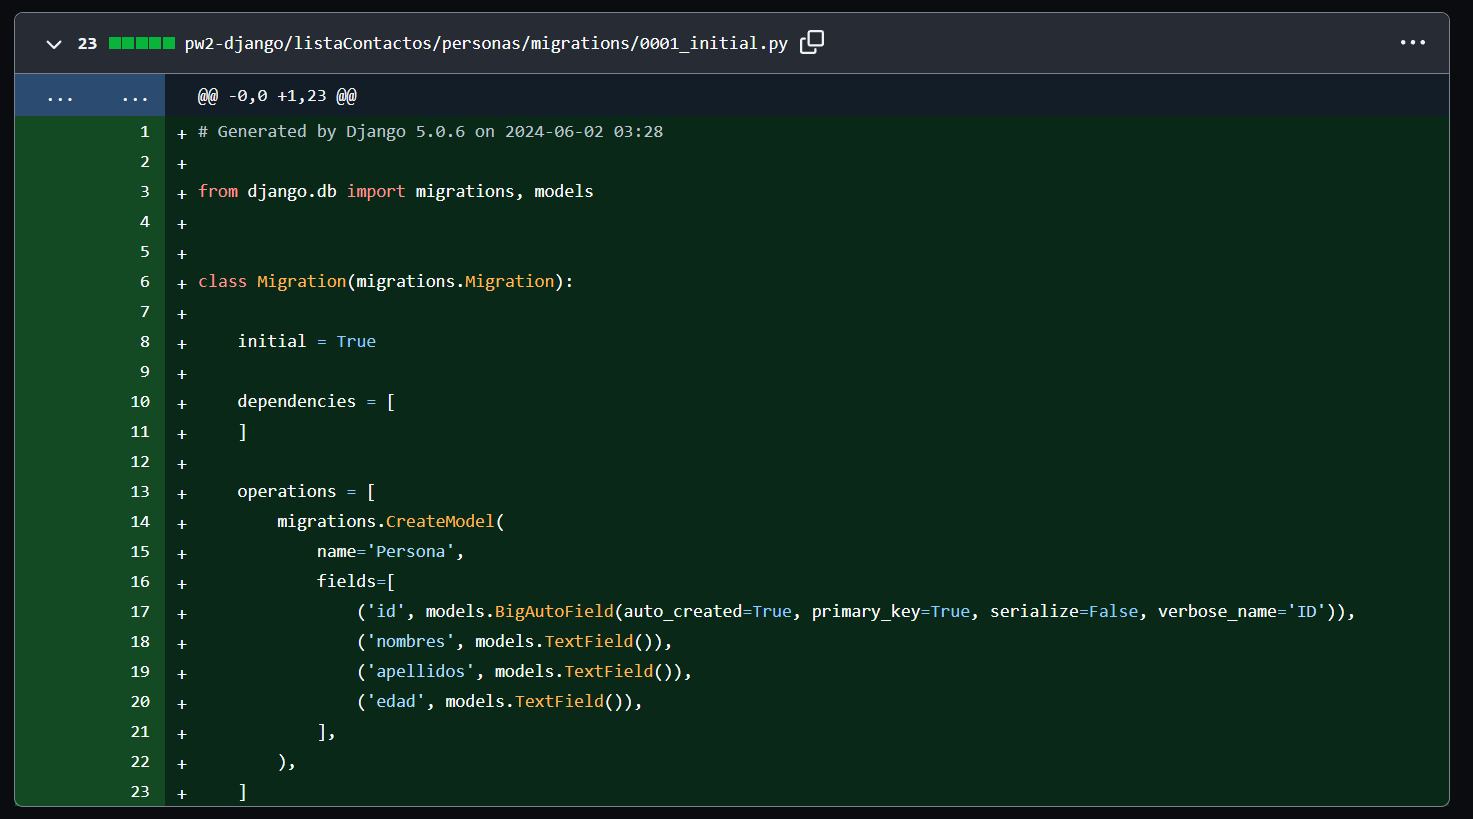
\includegraphics[width=0.7\linewidth]{img/Commit3.png}
            \caption{Migraciones aplicadas}
            \label{fig:enter-label}
        \end{figure}
        \end{itemize}
        
    %%%%%%%%%%%%%%%%%%%% ADMIN %%%%%%%%%%%%%%%%%%%%

    \section{Django Admin Site}
        \subsection{Creación de nuevo usuario}
        \begin{itemize}
            \item Para tener acceso al Admin Site de Django necesitamos crear un usuario administrador, en este paso se realiza el siguiente comando:
            
        \begin{lstlisting}[language=bash,caption={Comando para crear superusuario}][H]
        $ python manage.py createsuperuser jhonatan
        \end{lstlisting}
        
            \item Dentro de la consola, designamos los datos que tendrá nuestro usuario, en mi caso decidí llenarlo de la siguiente forma:
            
        \begin{lstlisting}[language=bash,caption={Creando superusuario}][H]
        $ python manage.py createsuperuser
            Nombre de usuario: jhonatan
            Direccion de correo electronico:
            Password: jbenja123
            Password (again): jbenja123
        \end{lstlisting}

        \subsection{Acceso a Django Admin Site}
            \item Tras este paso, se puede acceder al sitio administrativo de Django con el usuario y contraseña que se acaban de crear en \url{http://127.0.0.1:8000/admin/}:

        \begin{figure}[H]
            \centering
            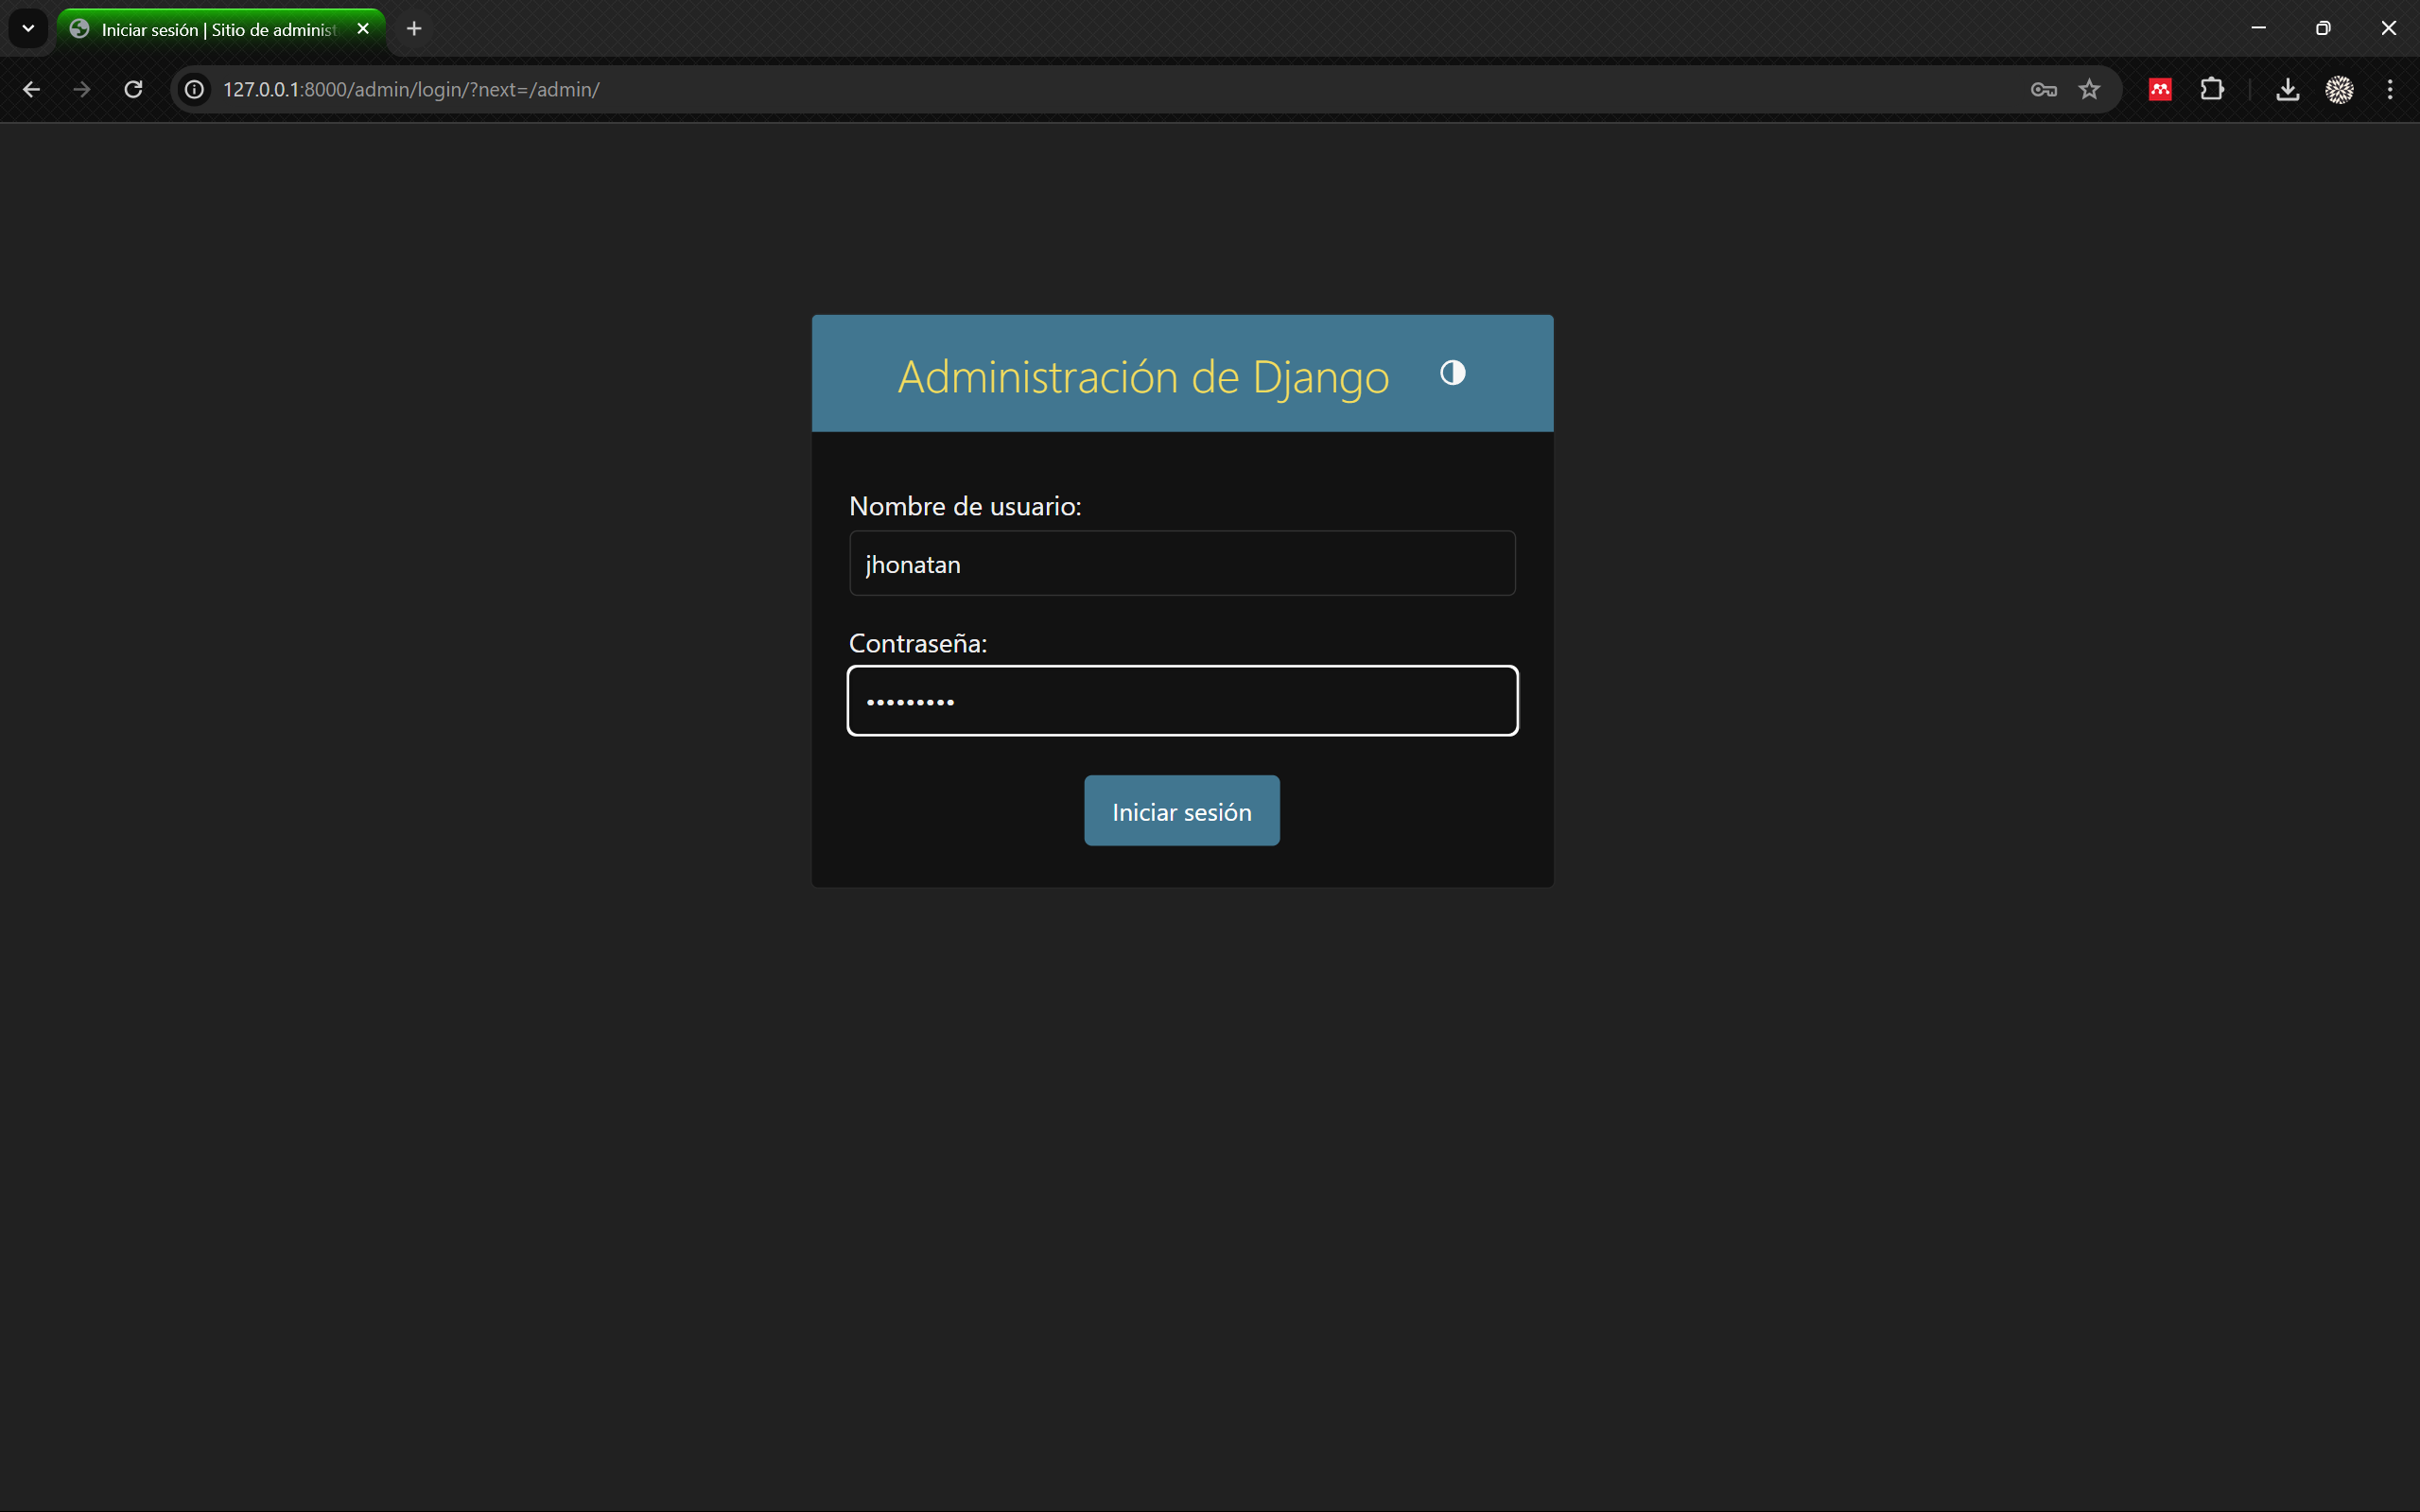
\includegraphics[width=1\linewidth]{img/Admin_login.png}
            \caption{Inicio de sesión}
            \label{fig:enter-label}
        \end{figure}
        
            \item Finalmente, al acceder al sitio administrativo de Django, se muestra la información sobre los usuarios y grupos registrados hasta ahora:
            
        \begin{figure}[H]
            \centering
            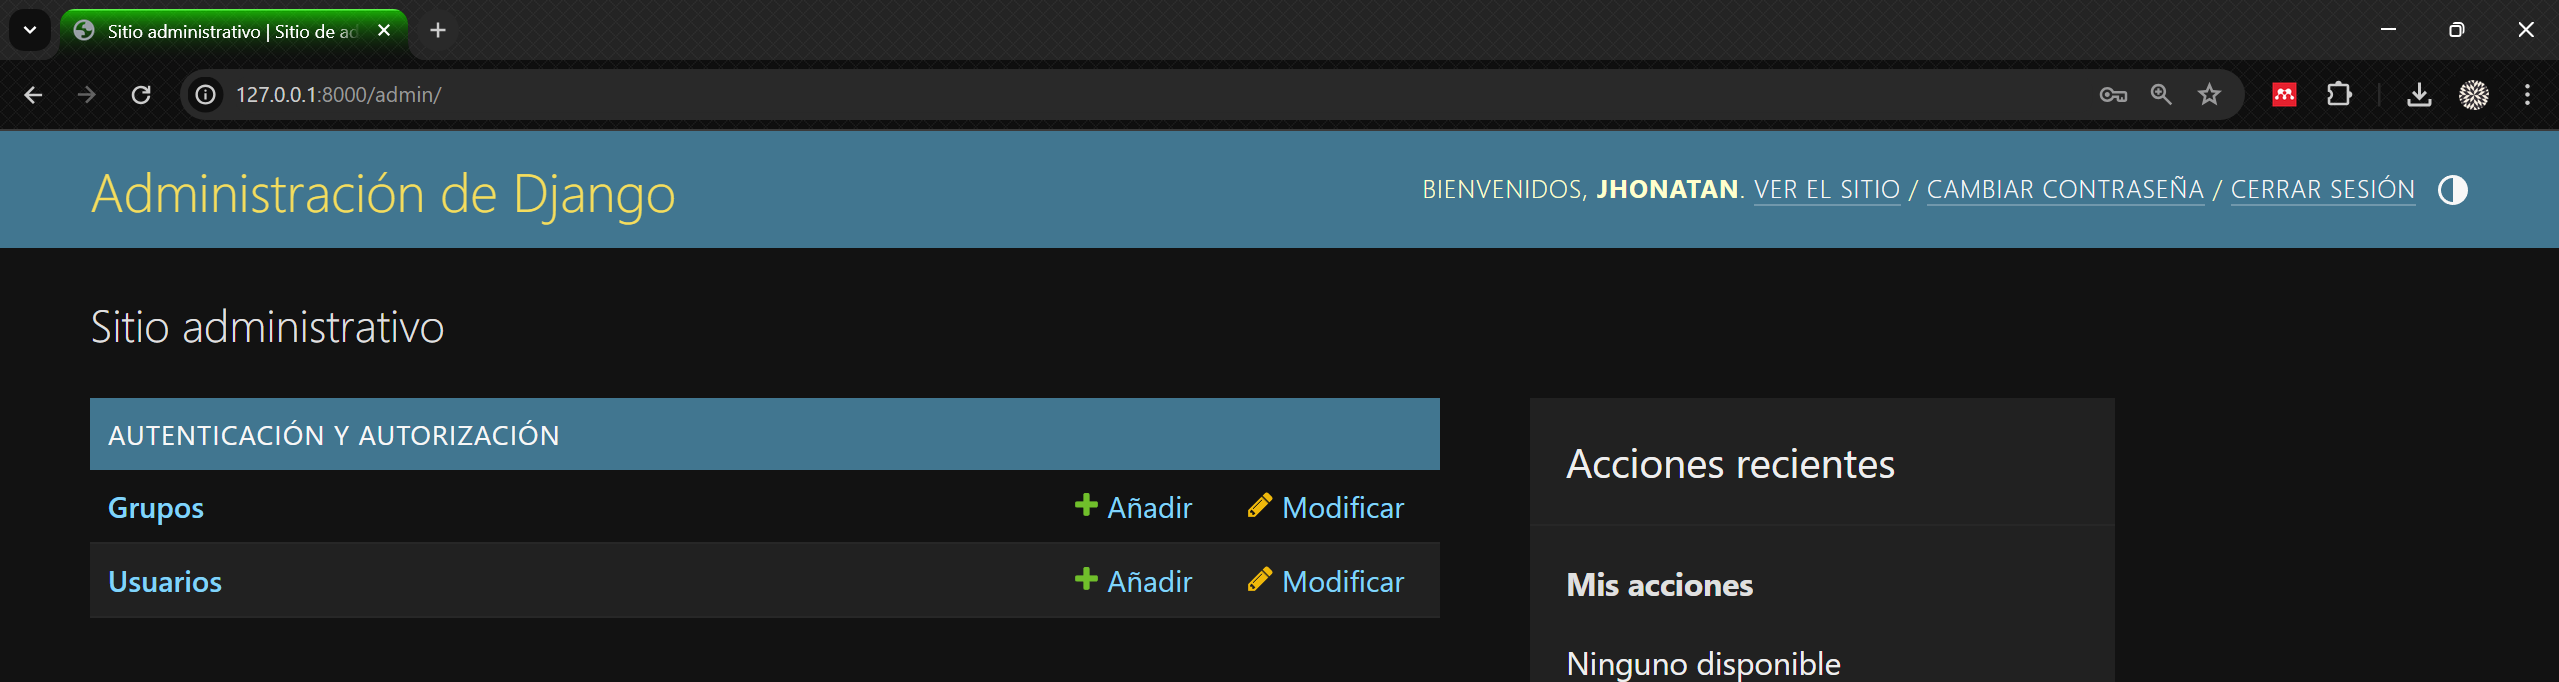
\includegraphics[width=1\linewidth]{img/Admin_site.png}
            \caption{Django Admin Site}
            \label{fig:enter-label}
        \end{figure}
            
        \subsection{Registro de modelos}
            \item El sitio administrativo es capaz de mostrar los modelos, sin embargo aquí no aparecen, en las diapositivas se sigue un paso simple para solucionarlo.
            \item Cuando se crean los modelos, se necesita registrarlos en el archivo admin.py de la aplicación en la que se crearon, es este caso, accedemos al de personas:
        \begin{lstlisting}[language=bash,caption={Ingresando a admin.py}][H]
        $ vim personas/admin.py
        \end{lstlisting}

            \item Aquí importamos el módulo de la clase que creamos antes en models.py de personas, luego lo registramos en el admin.site:

        \begin{lstlisting}[language=Python, caption={Registro del modelo Persona}]
        from django.contrib import admin
        
        # Register your models here.
        from .models import Persona
        
        admin.site.register(Persona)
        \end{lstlisting}
            \item Así se registró el cambio del archivo en el commit realizado:
        \begin{figure}[H]
            \centering
            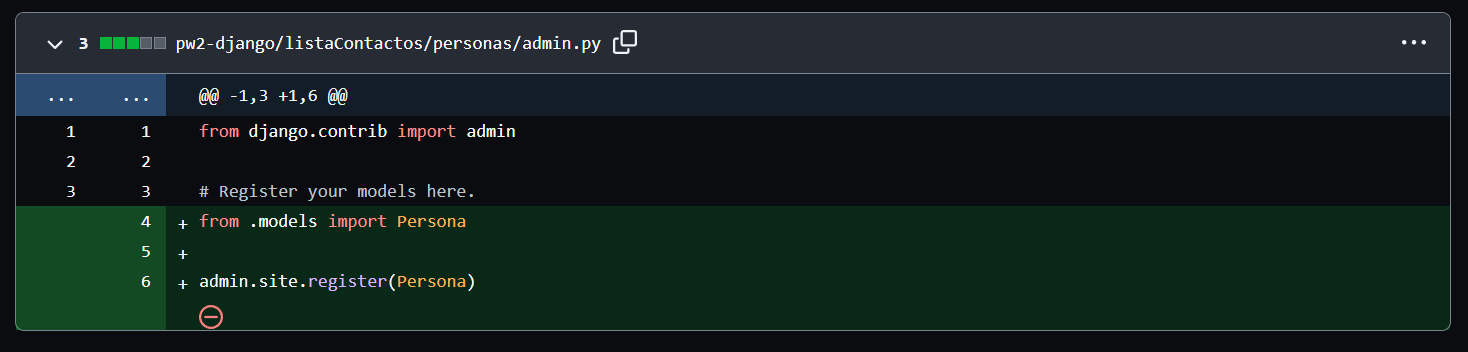
\includegraphics[width=1\linewidth]{img/Commit4.png}
            \caption{Commit de admin.py}
            \label{fig:enter-label}
        \end{figure}
            \item Entonces, tras esto, al reiniciar el servidor y volver a acceder al sitio administrativo de Django, encontraremos el acceso a la tabla generada desde el modelo Persona que creamos en el proyecto, curiosamente con el nombre en plural:
        \begin{figure}[H]
            \centering
            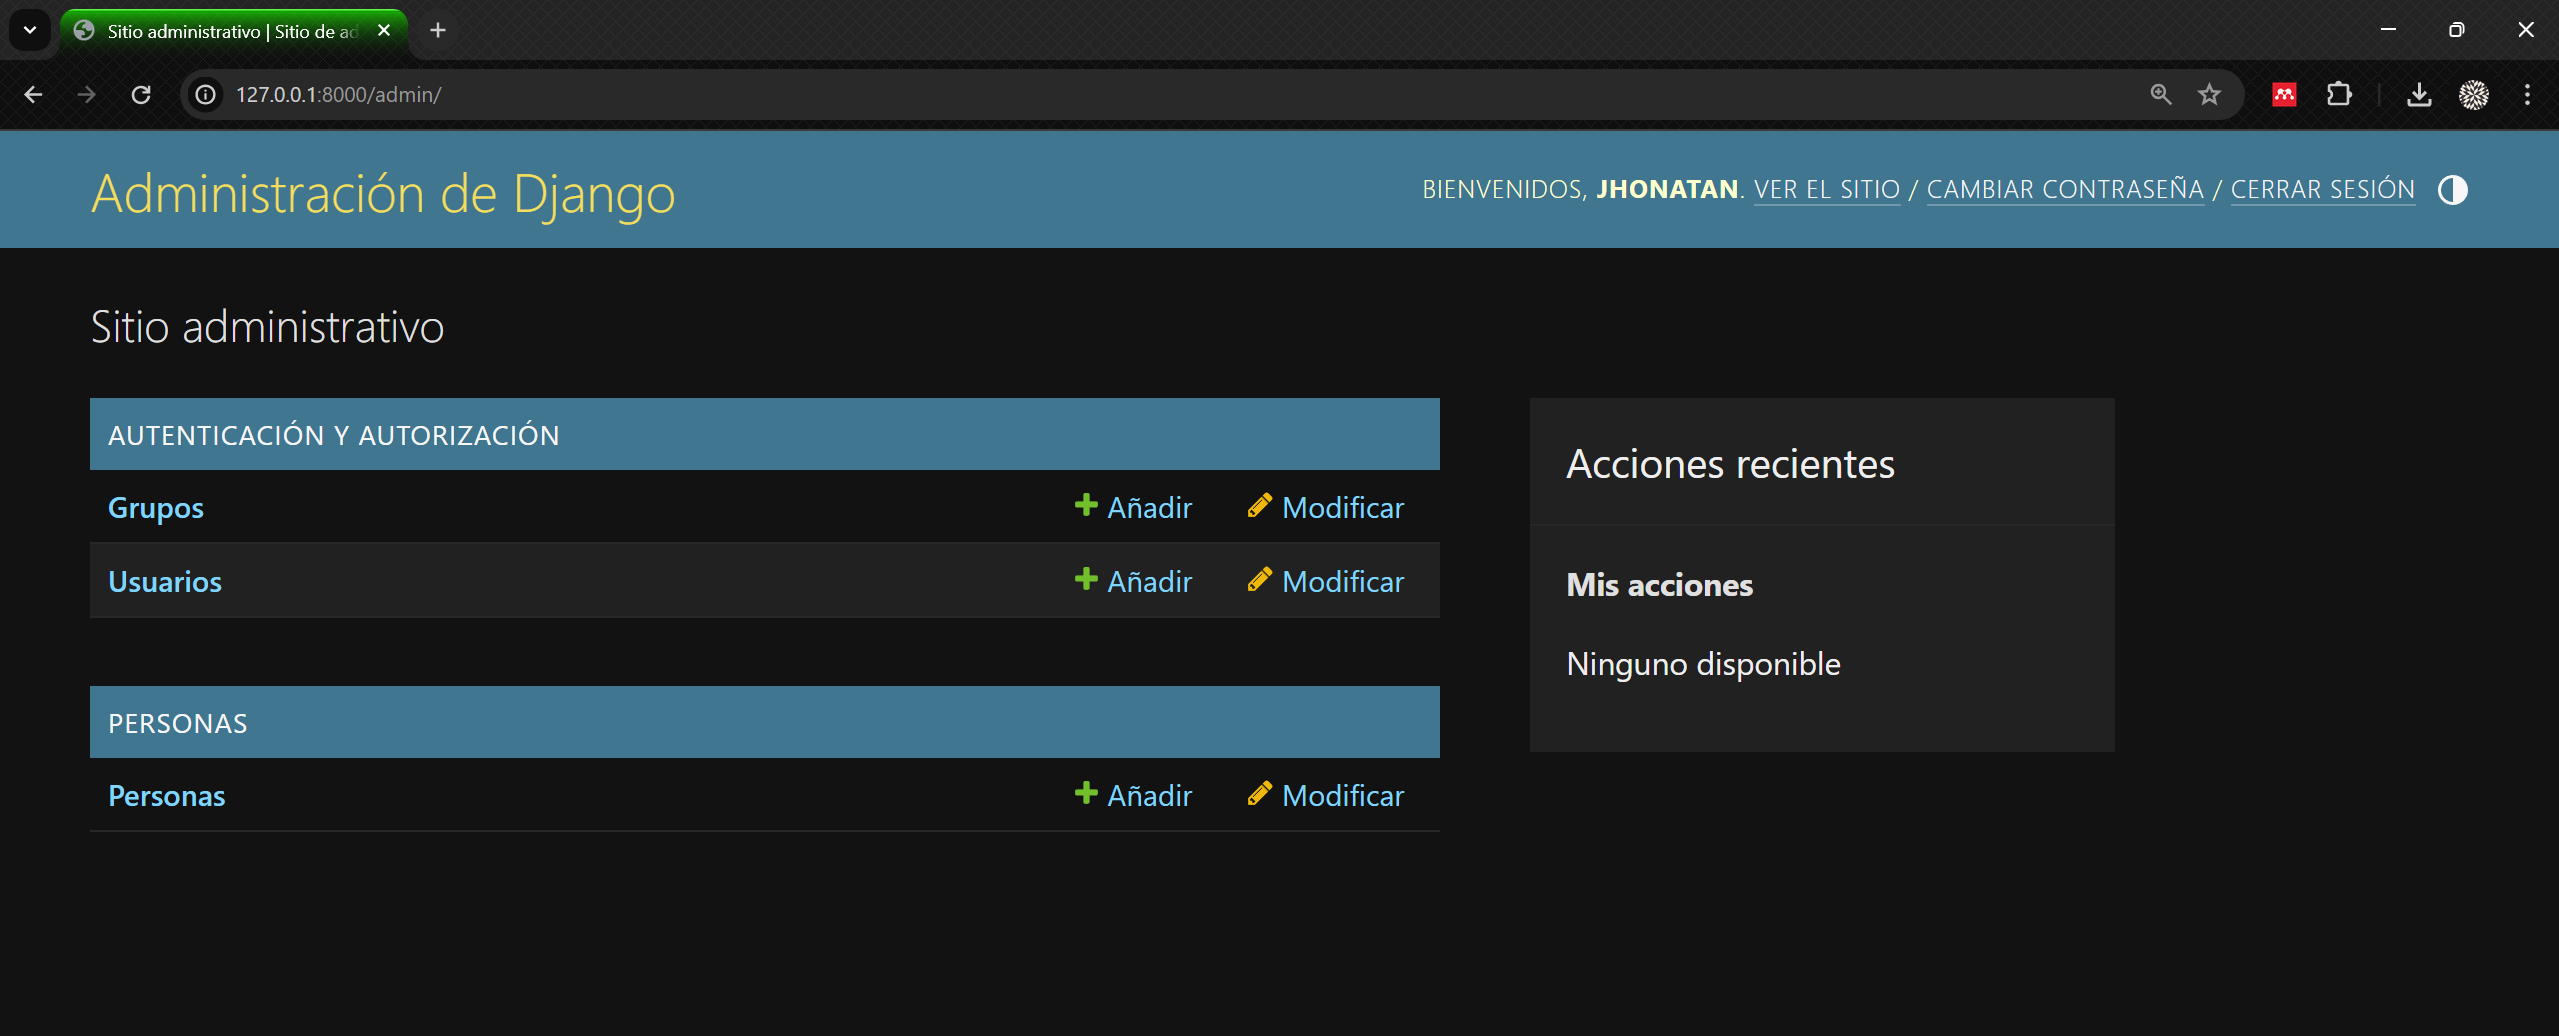
\includegraphics[width=1\linewidth]{img/Admin_site2.png}
            \caption{Django Admin Site (Con el modelo Persona)}
            \label{fig:enter-label}
        \end{figure}
            \item Desde este sitio es posible gestionar fácilmente los datos que se registran en el modelo, esto porque permite añadir, eliminar y modificar entradas en general.
        \end{itemize}

    %%%%%%%%%%%%%%%%%%%% PYTHON SHELL %%%%%%%%%%%%%%%%%%%%

    \section{Crear objetos en Python Shell}
        \begin{itemize}
            \item Además de la facilidad de crear objetos desde el sitio administrativo de Django, es posible agregar objetos desde el Shell de Python, para acceder a este se ejecuta lo siguiente:


        \begin{lstlisting}[language=bash,caption={Ingresando a Python Shell}][H]
        $ python manage.py shell
        \end{lstlisting}
            \item Una vez dentro del shell, se procede a realizar una serie de pasos; Se importa el módulo de la clase Persona, se revisa la cantidad de objetos creados en este modelo, se crea uno nuevo con la información del profesor Alfredo Paz Valderrama y se hace un nuevo llamado para confirmar la existencia del nuevo objeto creado:

        \begin{lstlisting}[language=bash,caption={Creación de un nuevo objeto desde el shell}][H]
        >>> from personas.models import Persona
        >>> Persona.objects.all()
        <QuerySet []>
        >>> Persona.objects.create(nombres="Alfredo", apellidos="Paz Valderrama", edad="23")
        <Persona: Persona object (1)>
        >>> Persona.objects.all()
        <QuerySet [<Persona: Persona object (1)>]>
        >>> exit()
        \end{lstlisting}
            \item Entonces, si se vuelve a iniciar el servidor, y nos dirigimos hacia el sitio de administración, podemos revisar su existencia también:
        \begin{figure}[H]
            \centering
            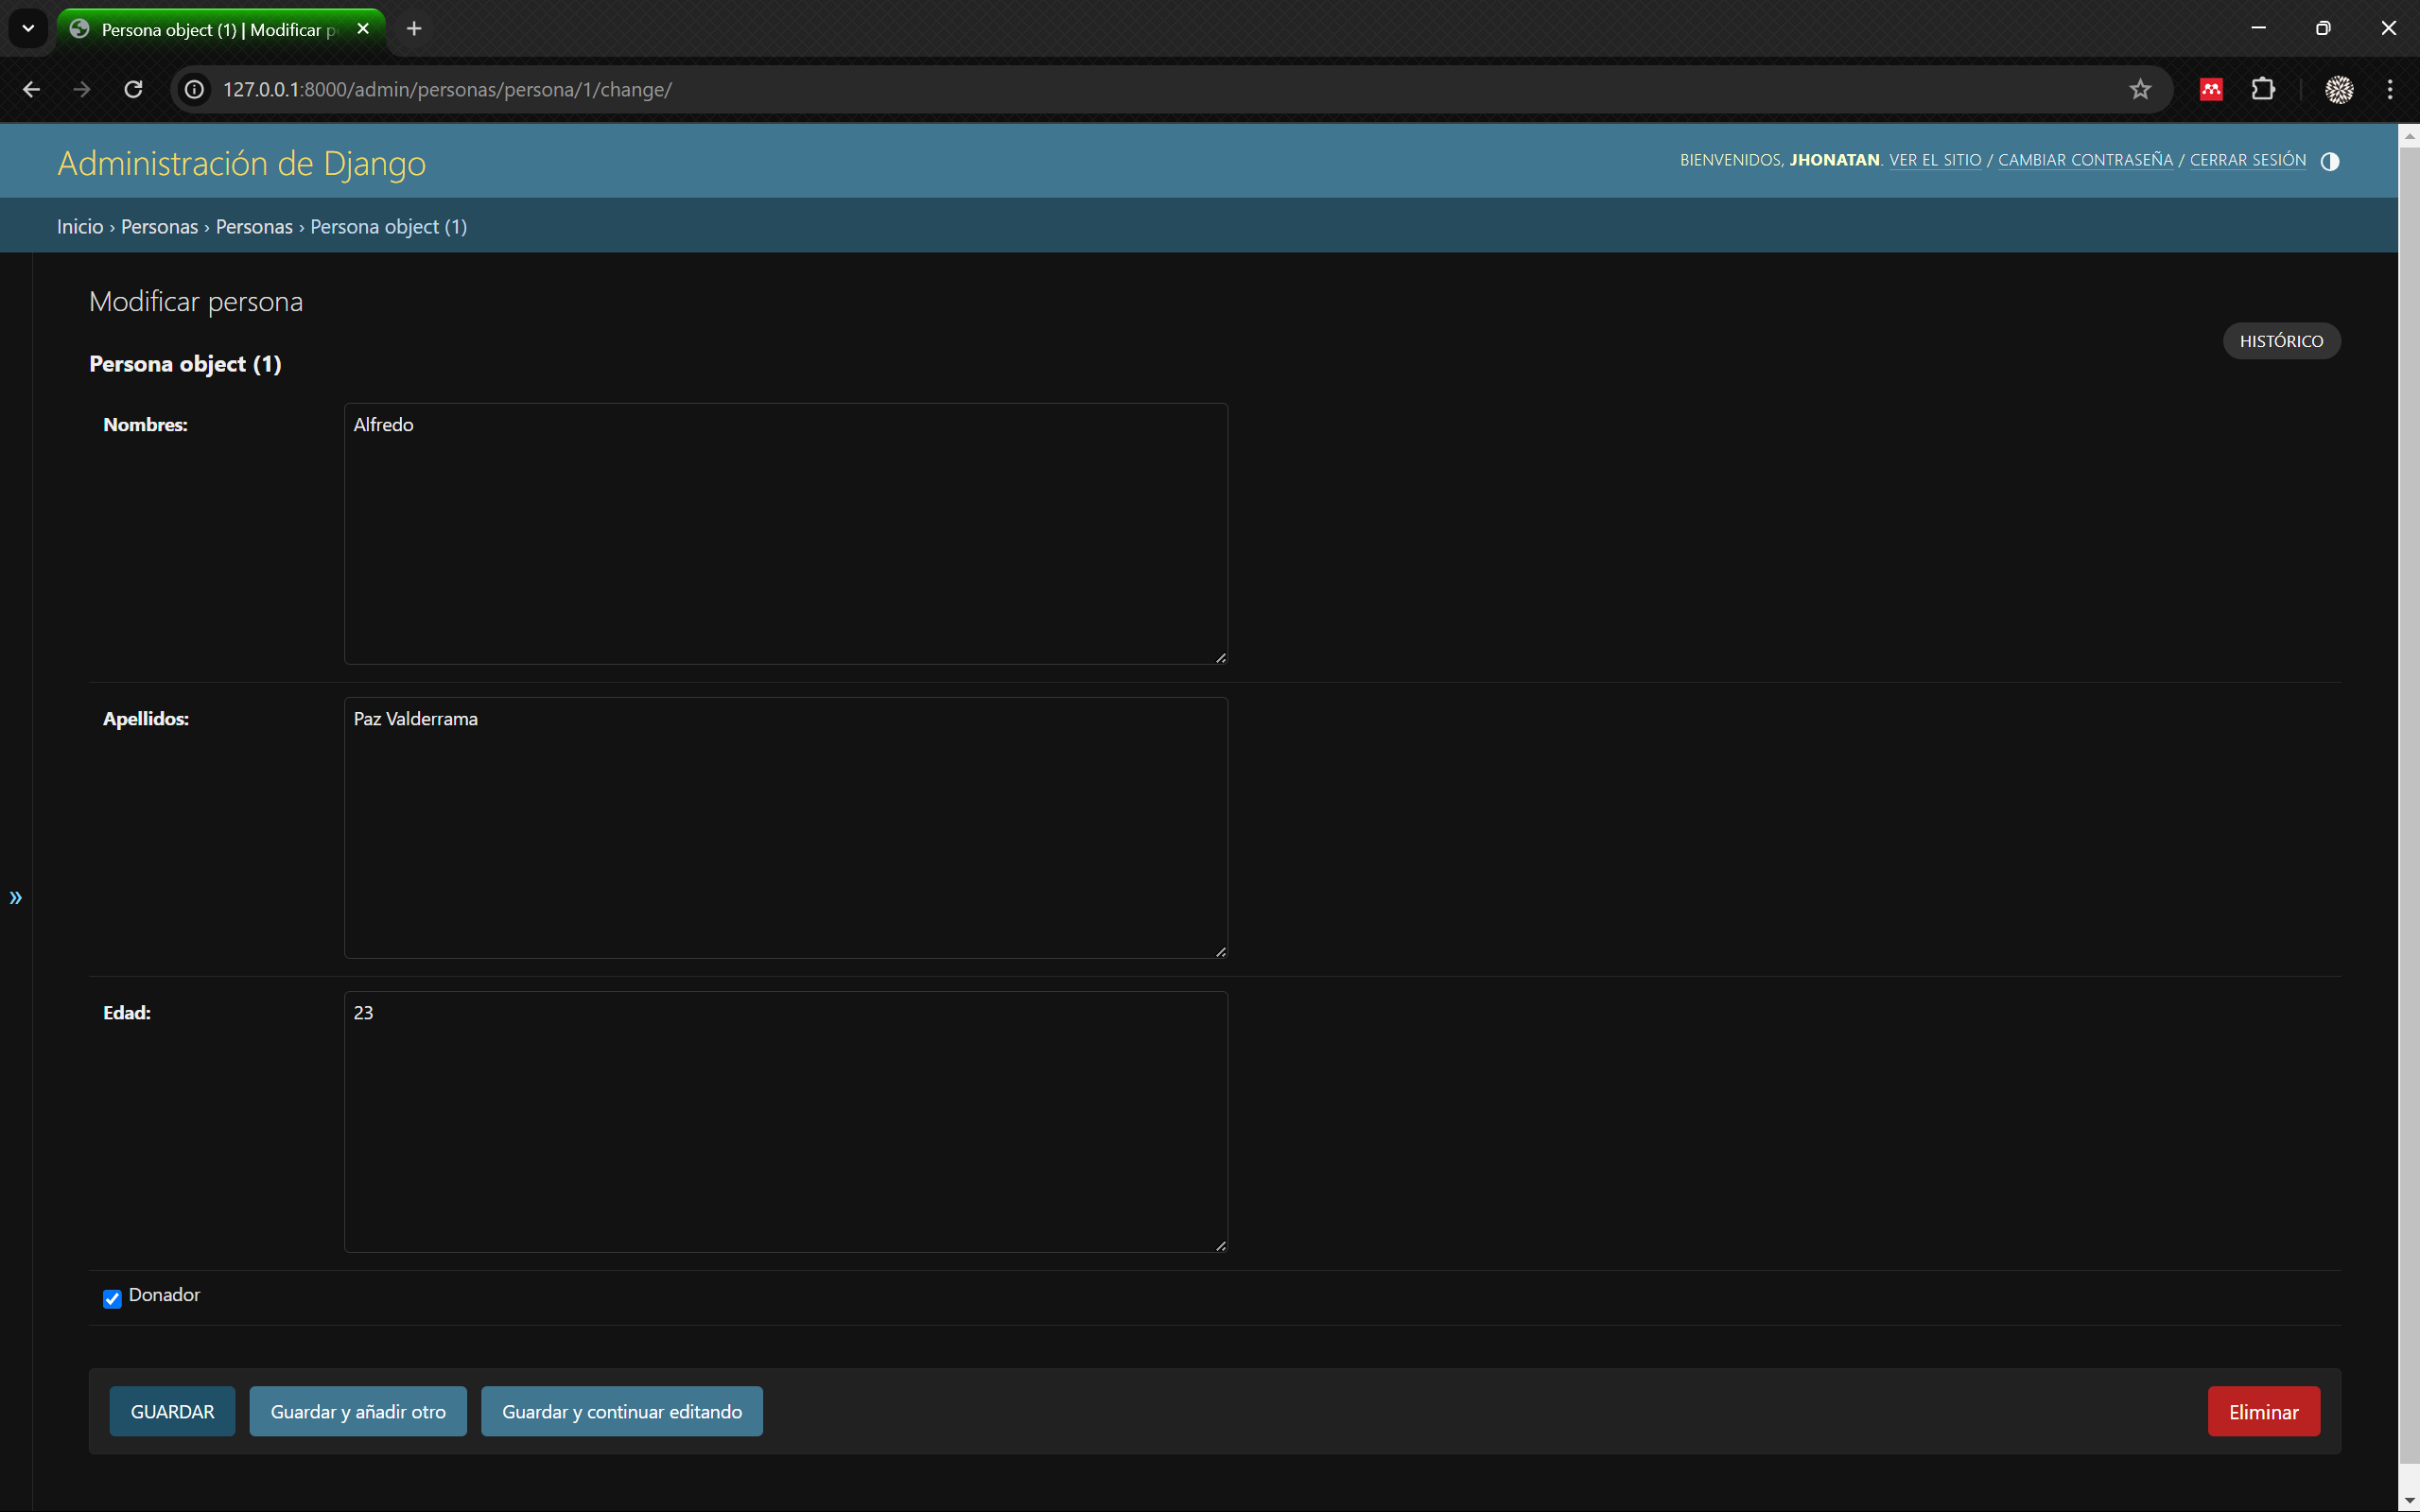
\includegraphics[width=1\linewidth]{img/Persona1.png}
            \caption{Django Admin Site (Persona 1)}
            \label{fig:enter-label}
        \end{figure}
        \end{itemize}

    \section{Captura de pantalla de commits}
        \begin{itemize}
            \item Como último paso de la actividad se ejecuta este comando para obtener el historial de los commits realizados en la actividad y le tomamos una captura:
        \begin{lstlisting}[language=bash,caption={Historial de commits}][H]
        $ git log --graph --pretty=oneline --abbrev-commit --all
        \end{lstlisting}
        \begin{figure}[H]
            \centering
            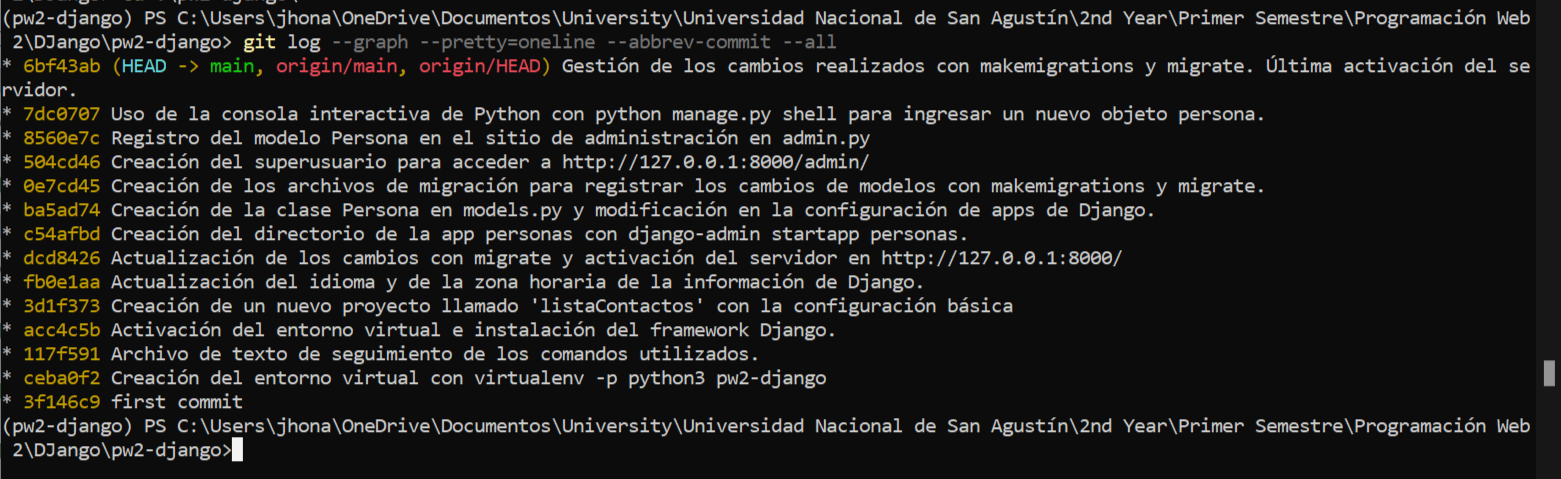
\includegraphics[width=1\linewidth]{img/Captura.png}
            \caption{Captura del historial de commits}
            \label{fig:enter-label}
        \end{figure}
        \end{itemize}
    \clearpage
    
    %%%%%%%%%%%%%%%%%%%% TREE DEL LABORATORIO %%%%%%%%%%%%%%%%%%%%
        
    \section{Estructura del trabajo}
        \begin{itemize}	
            \item El contenido que se entrega en esta práctica es el siguiente:
        \end{itemize}

        \begin{lstlisting}[style=ascii-tree]
        pw2-django/
        |--- Informe01
        |   |--- img
        |   |   |--- Admin_login.png
        |   |   |--- Admin_site.png
        |   |   |--- Admin_site2.png
        |   |   |--- Captura.png
        |   |   |--- Commmit1.png
        |   |   |--- Commmit2.png
        |   |   |--- Commmit3.png
        |   |   |--- Commmit4.png
        |   |   |--- Django_site.png
        |   |   |--- logo_abet.png
        |   |   |--- logo_episunsa.png
        |   |   |--- logo_unsa.jpg
        |   |   |--- Persona1.png
        |   |--- Informe_Django01.pdf    
        |   |--- Informe_Django01.tex
        |--- listaContactos
        |   |--- listaContactos
        |   |   |---__init__.py
        |   |   |--- asgi.py
        |   |   |--- settings.py
        |   |   |--- urls.py
        |   |   |--- wsgi.py
        |   |   |--- personas
        |   |   |   |--- migrations
        |   |   |   |   |--- 001_initial.py
        |   |   |   |   |--- __init__.py
        |   |   |   |--- __init__.py
        |   |   |   |--- admin.py
        |   |   |   |--- apps.py
        |   |   |   |--- models.py
        |   |   |   |--- tests.py
        |   |   |   |--- views.py
        |   |   |--- db.sqlite3
        |   |   |--- manage.py
        |   |--- Comandos.txt
        |--- .gitignore
        |--- README.md
        \end{lstlisting}
    \clearpage
    %%%%%%%%%%%%%%%%%%%% PREGUNTAS DEL INFORME %%%%%%%%%%%%%%%%%%%%
        
    \section{Preguntas:}
        \subsection{¿Qué archivos se modificaron al hacer makemigrations y migrate?}
        \begin{itemize}
            \item Se modifican los archivos dentro de la carpeta migrations.
            \item De manera más detallada, con el primero 'makemigrations', se detectan los cambios en los modelos de Django (definidos en models.py) y crea archivos de migración correspondientes en la carpeta migrations de cada aplicación. Estos archivos tienen nombres como 0001\_initial.py, 0002\_alter.py, etc., y contienen clases que heredan de django.db.migrations.Migration. Representan los pasos necesarios para aplicar (o deshacer) los cambios en la base de datos cada vez que modificamos los modelos.
            \item Luego, con 'migrate', se aplica o deshace las migraciones basadas en los archivos de migración. Actualiza la base de datos para que coincida con el estado actual de los modelos y mantiene un registro de las migraciones aplicadas en una tabla especial llamada django\_migrations. Aunque no modifica los archivos del código fuente, es responsable de actualizar la estructura de la base de datos (por ejemplo, creando o modificando tablas). 
        \end{itemize}

        \subsection{¿Qué archivos se modificaron al agregar personas?}
        \begin{itemize}	
            \item Al agregar nuevas entradas a la base de datos, como objetos del modelo Persona, no se modificaron archivos dentro del proyecto. En su lugar, aprendí que Django utiliza su Object-Relational Mapper (ORM) para generar y ejecutar consultas SQL que insertan los nuevos datos en la tabla correspondiente. Por ejemplo, con el panel de administración configurado, puedo agregar personas a través de una interfaz gráfica, y solo realiza inserciones en la base de datos sin modificar directamente ningún archivo mas que este.
        \end{itemize}

        %%%%%%%%%% RÚBRICA %%%%%%%%%%

        %\clearpage

	\section{\textcolor{red}{Rúbricas}}
	
	\subsection{\textcolor{red}{Entregable Informe}}
	\begin{table}[H]
		\caption{Tipo de Informe}
		\setlength{\tabcolsep}{0.5em} % for the horizontal padding
		{\renewcommand{\arraystretch}{1.5}% for the vertical padding
		\begin{tabular}{|p{3cm}|p{12cm}|}
			\hline
			\multicolumn{2}{|c|}{\textbf{\textcolor{red}{Informe}}}  \\
			\hline 
			\textbf{\textcolor{red}{Latex}} & \textcolor{blue}{El informe está en formato PDF desde Latex,  con un formato limpio (buena presentación) y facil de leer.}   \\ 
			\hline 	
		\end{tabular}
	}
	\end{table}
	
	\clearpage
	
	\subsection{\textcolor{red}{Rúbrica para el contenido del Informe y demostración}}
	\begin{itemize}			
		\item El alumno debe marcar o dejar en blanco en celdas de la columna \textbf{Checklist} si cumplio con el ítem correspondiente.
		\item Si un alumno supera la fecha de entrega,  su calificación será sobre la nota mínima aprobada, siempre y cuando cumpla con todos lo items.
		\item El alumno debe autocalificarse en la columna \textbf{Estudiante} de acuerdo a la siguiente tabla:
	
		\begin{table}[ht]
			\caption{Niveles de desempeño}
			\begin{center}
			\begin{tabular}{ccccc}
    			\hline
    			 & \multicolumn{4}{c}{Nivel}\\
    			\cline{1-5}
    			\textbf{Puntos} & Insatisfactorio 25\%& En Proceso 50\% & Satisfactorio 75\% & Sobresaliente 100\%\\
    			\textbf{2.0}&0.5&1.0&1.5&2.0\\
    			\textbf{4.0}&1.0&2.0&3.0&4.0\\
    		\hline
			\end{tabular}
		\end{center}
	\end{table}
	\end{itemize}
	
	\begin{table}[H]
		\caption{Rúbrica para contenido del Informe y demostración}
		\setlength{\tabcolsep}{0.5em} % for the horizontal padding
		{\renewcommand{\arraystretch}{1.5}% for the vertical padding
		%\begin{center}
		\begin{tabular}{|p{2.7cm}|p{7cm}|x{1.3cm}|p{1.2cm}|p{1.5cm}|p{1.1cm}|}
			\hline
    		\multicolumn{2}{|c|}{Contenido y demostración} & Puntos & Checklist & Estudiante & Profesor\\
			\hline
			\textbf{1. GitHub} & Hay enlace URL activo del directorio para el  laboratorio hacia su repositorio GitHub con código fuente terminado y fácil de revisar. &2 &X &2 & \\ 
			\hline
			\textbf{2. Commits} &  Hay capturas de pantalla de los commits más importantes con sus explicaciones detalladas. (El profesor puede preguntar para refrendar calificación). &4 & X& 3& \\ 
			\hline 
			\textbf{3. Código fuente} &  Hay porciones de código fuente importantes con numeración y explicaciones detalladas de sus funciones. &2 &X &2 & \\ 
			\hline 
			\textbf{4. Ejecución} & Se incluyen ejecuciones/pruebas del código fuente  explicadas gradualmente. &2 &X &2 & \\ 
			\hline			
			\textbf{5. Pregunta} & Se responde con completitud a la pregunta formulada en la tarea.  (El profesor puede preguntar para refrendar calificación).  &2 &X &2 & \\ 
			\hline	
			\textbf{6. Fechas} & Las fechas de modificación del código fuente estan dentro de los plazos de fecha de entrega establecidos. &2 &X &2 & \\ 
			\hline 
			\textbf{7. Ortografía} & El documento no muestra errores ortográficos. &2 &X &2 & \\ 
			\hline 
			\textbf{8. Madurez} & El Informe muestra de manera general una evolución de la madurez del código fuente,  explicaciones puntuales pero precisas y un acabado impecable.   (El profesor puede preguntar para refrendar calificación).  &4 & X& 4& \\ 
			\hline
			\multicolumn{2}{|c|}{\textbf{Total}} &20 & &19 & \\ 
			\hline
		\end{tabular}
		%\end{center}
		%\label{tab:multicol}
		}
        \end{table}
	
\clearpage

\section{Referencias}
\begin{itemize}			
        \item \url{https://www.w3schools.com/django/}
        \item \url{https://docs.djangoproject.com/es/5.0/intro/tutorial01/}
        \item \url{https://github.com/mdn/django-locallibrary-tutorial/blob/main/.gitignore}
        \item \url{https://developer.mozilla.org/en-US/docs/Learn/Server-side/Django/development_environment}
\end{itemize}	
	
%\clearpage
%\bibliographystyle{apalike}
%\bibliographystyle{IEEEtranN}
%\bibliography{bibliography}
			
\end{document}